% \documentclass[10pt,twocolumn,letterpaper]{article}
\documentclass[10pt,phd,a4paper,oneside]{article}
% \documentclass{article}
\usepackage[utf8]{inputenc}
\usepackage{natbib}
\usepackage{graphicx}
\usepackage[english]{babel}

\usepackage{listings}
\usepackage{xcolor}

\definecolor{codegreen}{rgb}{0,0.6,0}
\definecolor{codegray}{rgb}{0.5,0.5,0.5}
\definecolor{codepurple}{rgb}{0.58,0,0.82}
\definecolor{backcolour}{rgb}{0.95,0.95,0.92}

\lstdefinestyle{pythonCode}{
backgroundcolor=\color{backcolour},
commentstyle=\color{codegreen},
keywordstyle=\color{magenta},
numberstyle=\tiny\color{codegray},
stringstyle=\color{codepurple},
basicstyle=\ttfamily\footnotesize,
breakatwhitespace=false,
breaklines=true,
captionpos=b,
keepspaces=true,
numbers=false,
numbersep=5pt,
showspaces=false,
showstringspaces=false,
showtabs=false,
tabsize=2
}

\lstset{style=pythonCode}

%Import the natbib package and sets a bibliography  and citation styles
\bibliographystyle{abbrvnat}
% \bibliographystyle{abbrv}
% \setcitestyle{author,open={((},close={))}}


\title{Investigating implementing neural network architectures fore video classification}
\author{Olubunmi Aworanti}
\date{}
% \institution{University College London}


\begin{document}

    \begin{abstract}
        This paper investigates the design and building of different neural network architectures for video classification using tensorflow and the keras API. It begins by constructing a CNN Neural network architecture as described in \citep{KarpathyCVPR14}, using the keras API and tensorflow packages in python to build the required layer and models. these models where trained using the tensorflow UCF101 dataset. Finally it discusses minor adjustments made on model the performance and problems found with constructing and running these models.
    \end{abstract}

    \maketitle

    \section{Introduction}
    % this sounds like a summary rather than an introduction
    In past few years, with the increase in large labelled datasets such as the Imagenet dataset as discussed in \citep{JiaDeng2009IAlh} which is an image dataset organized according to the WordNet hierarchy where a wordnet is a meaningful concept which could also be described by multiple words or word phrases which are called a "synset". In the Imagnet dataset, WordNet contains more than 100,000 synsets, where nouns are the majority of about 80,000 plus. ImageNet aims to provide an average of 1000 images per each synset with the goal of offering tens of millions of images per WordNet. For video data of recent exist the YouTube-8M dataste as dicusssed in \citep{45619}, which a largest multi-label video classification dataset, composed of about 8 million videos for Youtube annotated with a vocabulary of 4803 visual entities. One intresting fact about the Youtube-SM dataset is that a Deep CNN pre-trained on ImageNet was also used to extract the hidden representation immediately prior to the classification layer showing how the available of large datassets can lead to progress in others. Not only have these datasets lead to growth with other datasets but most importantly they have also lead to a rise of various machine learning algorithms used to solve a diverse set of problems. Not only has the increase in datasets helped with this growth but also the increase in the available frames works and libraries used to create these various algorithms. some of these frameworks and libraries used for machine learning include scikitlearn which is a python programming language based library with a long range of user friendly API's for creating machine learning algorithms. \citep{DBLP:journals/corr/BuitinckLBPMGNPGGLVJHV13} details the use of scikitlearn and its elegant APIs which has lead to a growth in implementation of models in the machine learning space. In the deep learning space, surveys such as \citep{Nguyen2019} have been taken on the available libraries and frameworks for deep learning with large datasets and the hardware requirements some of these frames works propose.\citep{Wang2019}, is another survey that details the more commonly used deep learning frame works developed by large software houses such as Google, Facebook, and Microsoft, and those developed by the open source community such as Caffe, Caffe2, Tensorflow, MXNet, CNTK, Torch, PyTorch,  MatconvNet, Matlab deep learning and Deep learning tool box, Deeplearning4j to name a few.
    For the purpose of this paper we will be looking at using Tensorflow and keras libraries and APIs with python as the programming language for building and using popular models.
    Where Tensorflow is a free and open-source software library developed by Google and released in November 2015 for dataflow and differentiable programming as described in \citep{8578572} and keras as dicussed in \citep{Lux:2019:OSC:3310195.3310202} is a high-level elegant neural networks API that provides tools for easy constructions of models. It also provides access to popular pre-trained models and it is capable of running on top of frameworks like TensorFlow, CNTK, or Theano.
    This paper will be looking to experiment with how to implement neural network architectures for video classification particularly looking into deep convolutional neural networks which have been applied to a large pool of visual tasks since the late 1980s as discussed in \citep{doi:10.1162neco_a_00990}.
    % maybe add here more on video classification and temporal issues
    % Although primary used for image classification this paper will also be looking at the




    \section{Related Work}

    % talk abour related work here on other models for video classification double check the pedistrain dection paper%
    There is vast range of problems in which convolutional neural network(CNNs) architectures are used, some of which are in the image classification space which include problems such as object detection for example in pedestrian detection \citep{TomeD2016DCNN} systems, to speech  recognition problems and also facial and body recognition systems which are items in the human emotion recognition and human interaction space \cite{knyazev2017convolutional} .They have also been used in natural language processing for example with modelling sentences as explained in \cite{Kalchbrenner_2014}.
    Most importantly, CNNs have also been used for video classification for example by using the codec as a spatio-temporal Activity Sensor on videos as described in \citep{ChadhaA2017VCWC}. Apart from convolutional neural networks there are other machine learning methods used for example bag of words models \citep{10.1007978-3-642-28493-9_34}, this can be based on using local visual descriptors, most common of these are histogram of oriented gradients (HOG), histogram of optical flow (HOF) and motion boundary histograms (MBH) descriptors which are very powerful for classification but also computationally expensive as described in \citep{Uijlings2015}. Other methods use recurrent neural networks(RNNs) which is also used in the natural language processing space and in general for sequence data. Since videos are essentially sequence data, RNNs can be used in theory however because RNNs are difficult to train on high-dimensional inputs due to the large input-to-hidden weight matrix there has been some difficulty using them, however there is additional research in the space that has lead to competitive results such as that described in \citep{yang2017tensortrain} which factorizes the input-to-hidden weight matrix using Tensor-Train decomposition to help with efficiency of training these models.
    % reference need for von Neumann bottleneck and https://cloud.google.com/blog/products/ai-machine-learning/what-makes-tpus-fine-tuned-for-deep-learning%
    Also when running these models apart from architecture one has to also consider processing hardware as evaluated in \citep{wang2019benchmarking} as this has an effect performance. Devices range (Central processing units) CPUs, which reads each instruction from the software hence has to store all calculaculations internally on memory. This memory access becomes the downside of CPU architecture called the von Neumann bottleneck because each CPU's Arithmetic Logic Units (ALU) executes calculation one by one, accessing the memory every time, limiting the total throughput and consuming significant energy. Another is the GPU(Graphical processing units which uses thousands of ALUs(about 2,500–5,000) in a processor of ALUs which means it can then execute thousands of multiplications and additions simultaneously. However it still suffers from the von Neumann bottleneck because For every  calculation in the thousands of ALUs, GPU it still needs to access shared memory to read and store intermediate calculation results. The most recent device of late is the Google designed, TPU (Tensor Processing Unit), which is designed as a matrix processor specialized for neural network work loads and is not as affected by the von Neumann bottleneck because its' primary task is matrix processing hence it consist of thousands of multipliers and adders connected to each other directly to form a large physical matrix called the systolic array architecture. Hence calculations naturally flow through the architecture reducing memory access during calculation and as a result it has a high computational throughput on neural network calculations with much less power consumption and smaller footprint.
    %   todo add how easy it is to implement to bring it all together

    %   such as there is a range of models typically used such as -----, videos can also be looked and complication of images in frames which simple convolutional networks can be use to classify together with methods used to take into account the temporal features.

    %   talk about vido clasification
    % This models have produced great results when it comes to image classification as discussed further in papers such as \citep{MISHKIN201711}. The use of convolutional neural networks doesn't stop in the computer vision field with image classification and video classification but also extends to tas well as physiological data, speech to name a few.

    % why tensor flow this is a good paper \citep{schrimpf2016i}

    % When looking to build most reasches beging by either devloping there own neural network and looking at the archetures of other. one of the issue faces is the the same computational pwoer and hypter paraametres found.


    \section{Overview}
    As mentioned previously this report looks to implement convolutional networks for video classification particularly looking at action labelled data, Where a convolutional neural network is simply a neural network that uses a convolution operation in place of a matrix multiple in atleast one of its layers as defined in \citep{Goodfellow-et-al-2016}. It also usually includes a pooling layer which is a applys a function that replaces an input a with a summary statistic of the nearby input.
    % explain convultional netweorks with pooling layer
    This project will begin by constructing models using the keras and the tensorflow API taking as an input each frame containing an image from the video then it will move on to use other architectures that take into account temporal features. The initial architectures will be based off those discussed in \citep{KarpathyCVPR14}, where different models are explored for large-scale video classification with convolutional neural networks. These models will be built using the python as the programming language  with the tensorflow framework. This project also looks to investigate popular pretrained models with the current software and hardware available.
    Another aim will be to explore the difficulties with recreating popular models with the current software and hardware at hand. It also aims to give an understanding from a software engineering prespective on how to begin with constructing these models.
    % with the future aim of exploring with emotion classification using image and video data. Something that has been explored in papers such as \cite{SUN201836}
    % explain f what a convutional neural network is here, talk about Alexnet
    % In order to get familiar with building neural networks, the first task involved  then understanding the structure and looking atthe performance of pretrained models CNN models readily available.

    \subsection{Implementation}
    % todo explain the clusters better
    Since the project required tensorflow and the keras API with python programming language, python 3.6 was used as it is the newer and more compatible python version from the legacy soon to be deprecated python 2.7. The initial coding environment set up was done using Anaconda which is a an open-source distribution for python and python libraries which are typically used for scientific computing. It also provides a distribution for R programming language. A benefit of anaconda is that it allows for multiple python environments and easy download of libraries and a very friendly user graphical interface as well as a command line interface.
    The tensorflow libraries which comes in two distribution one being the GPU enabled distribution with uses the GPU first by default to speed up certain processes then CPU and the other being the normal which runs simply on the CPU. The project initially began on a laptop with no GPU capacity, hence the tensorflow CPU package was installed.
    As mentioned briefly previously, Tensorflow uses a dataflow graph in which the nodes represent units of computation, and the edges represent the input data or the output data of the computation. This data flow allows for benefits such as the use of parallel computing for model, distributed execution through the use of explicit edges which allow for partitioning across multiple devices. It also improves compilation and generates faster code by allowing TensorFlow's XLA compiler use dataflow graph information. The dataflow graph is also language independ allowing for prtability between language.
    TensorFlow comes with a keras API within its libraries, this version of Keras supports the use of the datagraph unlike the readily available keras library hence it is there is no need to download keras separately in order to reap the benefits of te Tensorflow data flow.
    The project also initially began in a jupyter notebook environment which is an open sourced web-based interactive development environment used for a multitude of scientific research. An Empirical Study on Jupyter notebook as a tool for open science has also been taken as seen in \citep{Randles_2017}.  While on jupyter notebook, tensorflow was ran in eager mode which is a programming environment provided by tensorflow which evaluates operations from the dataflow graph immediately by not building computational graphs, hence allowing concrete values to be returned instead of constructing a graph to run later making debugging easier in such an interactive environment like jupyter notebook.
    Once familiar with the working of the Tensorflow environment, The models when then transferred into python scripts and then ran in the terminal then on the UCL cluster infrastructure using the interactive session, which allows for requesting nodes with different processing configuration. Using this interactive session to decide on what the clock time and hardware will be needed for script when ran in a batch job. The time needed to run each job was approximated based on the time taken for the first steps in the fist epoch from the interactive mode. Computing with GPU, CPU and parallel running we considered.

    % Rather building models from scracth the tensorflow package and keras  packages where used to construct the models and access the pre-trained models.

    \subsection{Datasets}
    Tensorflow also provides readily available pre-processed data sets for easy use. these datasets are available using the tensorflow dataset library. The Tensorflow dataset is a library that exposes publicly available datasets as numpy arrays, tensorflow dataset object and tensors. The range of datasets range from images to audio to text datasets.
    This project used the UCF101 dataset provided by this library which is an action recognition data set of realistic action videos, collected from YouTube, having 101 action categories \cite{soomro2012ucf101}. It contains about 13320 videos from 101 action categories, the videos in 101 action categories are grouped into 25 groups, where each group can consist of 4-7 videos of an action, videos from the same group may share some common features, such as similar background, similar viewpoint, etc.
    The action categories can be divided into five types which include Human-Object Interaction, Body-Motion Only, Human-Human Interaction , Playing Musical Instruments and Sports.
    Tensorflow also provides a train test split of the data where number of training examples are 9537 and the number of test examples are 3783.
    It also provides the functionality to take a custom spilt of the data and reduce the number of videos used for training. Each clip contains mutiple frames of 256x256x3.
    %todo crosscheck how youtube-8m download works%
    This UCF101 data set is also used in \citep{KarpathyCVPR14} to train models based off pretrained models trained with the larger data set of sports-1M  validation of the final models trained on the sport-1M dataset.
    Although most of links of the videos in the sports-1M dataset, which consists of over one million YouTube videos belonging to about 487 classes of sports is readily available on youtube for download there is a challenge of speed of model and with memory when it comes to downloading this large dataset. There is also the challenge were there is no clear copyright instruction for download applicable to all the videos. Hence the smaller UCF101 was decided to be used to recreate the models. It is also important to note that the sports-1M is also available as part youtube-8M datset. And although there is an API available to download youtube-8M as TensorFlow Record file, the sports-1M dataset cannot be easily  separated out of youtube-8M as it does not allow for access to specific videos. which would be a nice addition because the sport-1M dataset github page provides the list of videos included in the sport-1M dataset split into training and test datasets.

    % might be worth summaring the dataset used in karpathy's paper


    \subsection{Architectures}

    In Karpathy paper on Large-scale Video Classification with convolutional Neural Networks \citep{KarpathyCVPR14}, it discusses various models and explores approaches for fusing information over temporal dimension through the convolutional network and compares their performance. Using the UCF101 dataset and tensorflow, I will also explore recreating these models and apply newer techniques for optimization. The models which will be implemented are listed below. The structures of these models can be also be seen in figure \ref{fig:k_models} taken from \citep{KarpathyCVPR14}
    \begin{itemize}
        \item Single Frame: is loosely based on the Alexnet model \cite{NIPS2012_4824}, which was the winning model of the ImageNet challenge in 2012. Alexnet model takes in an input image of $224 \times 224 \times 3$, using the shorthand notation as described in \citep{KarpathyCVPR14}, the full architecture is $C(96, 11, 4)-N-P-C(256, 5, 1)-N-P-C(384, 3, 1)-C(384, 3, 1)-C(256, 3, 1)-P-F C(4096)-F C(4096)$, where $C(d, f, s)$, is a convolutional layer with d filters of spatial size $ f × f$, with a stride of $s$,  $FC(n)$ is a fully connected layer with n nodes, $N$ is local response normalization layer and P is the pooling layer. The single frame model from \cite{KarpathyCVPR14} follows the following architecture  $C(96, 11, 3)-N-P-C(256, 5, 1)-N-P-C(384, 3, 1)-C(384, 3, 1)-C(256, 3, 1)-P-F C(4096)-FC(4096)$ with the exception that it takes in an image of size $ 170 \times 170 \times 3$. The single frame also uses a max pooling is non-overlapping with size $2 \times 2$ rather than overlapping pooling of size $3x3$ and stride $2$ used in the Alexnet. This is an interesting difference that might have an effect on performance as the Alexnet paper suggest that gerrally they observed during training that models with overlapping pooling found it slightly more difficult to overfit.
        \item Early Fusion - This combines information across an entire time window immediately on the pixel level hence making the input size that of $11 \times 11 \times 3 \times T$ pixels, where T was 10 which is also the number of frames covered. The change in input shape also required a change to the first convolutional layer to use a filter size of $10 \times 11 \times 11$.
        \item Late Fusion: This uses two single frame networks, taking in about 15 frames apart and combining them at the fully connected layers
        \item Slow Fusion: Is a mix of both late and early fusion, slowly combing the temporal information over at each convolutional layer. The input is a clip containing 10 frames. The first convolution layer now consist of 4 parallel layers that each take in 4 frames out of this clip, The second convolutional layer consist of two parallel layers that combines the two outputs from the first while the third layer combines the output from the second layer
    \end{itemize}



    \begin{figure}
        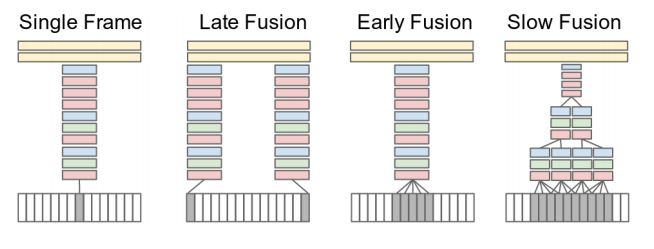
\includegraphics[width=\linewidth]{K_models.JPG}
        \caption{citep{KarpathyCVPR14} explored approaches for fusing information over
        temporal dimension through the network. Red, green and
        blue boxes indicate convolutional, normalization and pooling layers respectively \citep{KarpathyCVPR14}}
        \label{fig:k_models}
    \end{figure}
    There is a wide range of a pretrained convolution neural networks architectures particularly models for image classification trained on ImageNet dataset on the keras API. However there where a few explored as listed below.
    \begin{itemize}
        \item VGG19: as described in \citep{simonyan2014deep}, is quite a standard architecture that is made of a convolutional $3 \times3$ filters with a stride 2, followed by a $2\times2$ max-pool with a stride of 2.
        \item MobileNetV2: is a model created for mobile vision application available in keras. MobileNetV2\cite{Sandler_2018} makes an improvment from its predecessor MobileNetV1 \citep{howard2017mobilenets}, which uses depthwise separable convolution as efficient building blocks. However it introduces a linear bottlenecks between the layers, and a shortcut connections between the bottlenecks.
        \item Inception: this architecture \citep{Szegedy_2016} is made up of inception blocks which evaluate multiple multiple pooling layers of different dimensions then concatenate the results.
        \item ResNet: this architecture \citep{He_2016} is made up of residual blocks, which are a set of two layers that rather than going through the standard path of going from one activation layer to the next, addes the linear equation used to arrive at the activation value for the next layer. This is believed to have the benefit of helping with vanishing and exploding gradients to improve performance as the neural network gets deeper
    \end{itemize}


    \subsection{Coding}

    The coding began by first importing the tensorflor and tensorfloe dataset.

    \begin{lstlisting}[language=Python, caption=Importing tensorflow libaries]
        import tensorflow as tf
        import tensorflow_datasets as tfds
    \end{lstlisting}

    Using the tensorflow dataset libary allowed for easy loading of the UCF101 dataset as seen below. The libary also provides a default recommeneded train and test dataset. It also provided an information object detailing the labal and dataset size for the train and test size.

    \begin{lstlisting}[language=Python, caption=Loading UCF101 dataset]
        ucf101_dataset, ucf101_info = tfds.load(name="ucf101", with_info=True)
        ucf101_train , ucf101_test = ucf101_dataset["train"], ucf101_dataset["test"]
    \end{lstlisting}

    Custom python helper methods where used for the formatting of the images in the frame from $256 \times 256 \times 3$ to $170 \times170 \times 3$ as suggested in \citep{KarpathyCVPR14}. Most layers needed to build the model where present in the keras API. Most models where implemented using the keras sequential model which is the simplest model to implement as it is a simply a linear stack of layers as seen below. The single frame layer for example was implemented as a keras sequential model by passing in a list of layers as seen in \ref{singleFrame} note that this can also be implemented by using the the keras API add method to add in layers. More complex architectures such as the slow fusion layer used the keras functional API which uses the fact that a layers is a callable instance that can be called on a tensor and then returns a tensor to build multi-output and multi-input models like the slow and late fusion model.

    \begin{lstlisting}[language=Python, caption=Single Frame model implemetation, label=singleFrame]
        model = tf.keras.models.Sequential([
        tf.keras.layers.Conv2D(96, (11,11), strides=3 , activation='relu', input_shape=(170, 170, 3)),

        l.MyLRNLayer(),
        tf.keras.layers.MaxPooling2D(2, 2),
        tf.keras.layers.Conv2D(256, (5,5), strides=1, activation='relu'),

        l.MyLRNLayer(),
        tf.keras.layers.MaxPooling2D(2, 2),
        tf.keras.layers.Conv2D(384, (3,3), strides=1, activation='relu'),

        tf.keras.layers.Conv2D(384, (3,3), strides=1, activation='relu'),
        tf.keras.layers.Conv2D(256, (3,3), strides=1, activation='relu'),

        tf.keras.layers.MaxPooling2D(2,2),
        tf.keras.layers.Flatten(),

        tf.keras.layers.Dense(4096, activation='relu'),
        tf.keras.layers.Dense(4096, activation='relu'),
        tf.keras.layers.Dense(101, activation='softmax')
        ])
    \end{lstlisting}

    %todo more on the difference between LRN and batch normalization%
    Some custom layers where needed like the local response normalization layer as described in \citep{NIPS2012_4824}. This was because it was no longer available on the keras API. As the local response normalization is a non-trainable layer normalizes values in a feature map within a local making less adaptive. While its replacement batch normalization as discussed in \citep{ioffe2015batch} is a trainable normalization layer wich allows for a much higher learning rates and requires less care with initialization. Batch normalization in some cases is also said to eliminate the need for Dropout.
    Another benefit of the Keras API is how it allows for easy creation of a custom layers through inheritance from its keras layer class as seen in \ref{lrn}. Here since all the parameters of the LRN are fixed no training is required hence the layer is set to trainable false.
    This implementation also utilizes the tensorflow nn API which holds a functions that can be applied to tensor. Fortunately it also offers a local response normalization layer function calculation which returns the normalized tensor hence this was wrapped in the keras layer object so it can be used in  keras sequential model to implement the models.

    \begin{lstlisting}[language=Python, caption=Local response normalization layer implemetation, label=lrn]
        class MyLRNLayer(tf.keras.layers.Layer):
        def __init__(self, depth_radius=5,bias=1,alpha=1,beta=0.5, **kwargs):
        #         self.output_dim = output_dim
        self.depth_radius = depth_radius
        self.bias = bias
        self.alpha = alpha
        self.beta = beta
        super(MyLRNLayer, self).__init__(**kwargs)

        def build(self, input_shape):
        # Create a trainable weight variable for this layer.
        self.kernel = self.add_weight(name='kernel',
        shape=(None),
        initializer='uniform',
        trainable=False)
        super(MyLRNLayer, self).build(input_shape)  # Be sure to call this at the end

        def call(self, x):
        return tf.nn.local_response_normalization(x,self.depth_radius,self.bias,self.alpha,self.beta)
    \end{lstlisting}


    \subsection{Optimizations}

    As mentioned previous, Karpathy's models uses the local response normalization \cite{ROBINSON20071631} also used in the alexnet paper\cite{NIPS2012_4824}, however this normalization is now considered obsolete and the batch normalization \cite{ioffe2015batch} is the new standards normalization layer with some optimization benefits. Hence the models were also re-constructed using the recommended batch normalization in order to compare the results.

    Karpathy's paper also using downpour stochastic gradient descents with multiple distributed systems because the dataset used is much smaller than that used in \citep{KarpathyCVPR14}. It was decided to use the standardd stochastic gradient descents optimization offered by the keras API using the parameter values from \citep{KarpathyCVPR14} which set a learning rate of $1e^-3$, momentum of 0.9 and decay of $0.0005$. How this is was implemented can be seen in \ref{sdgKeras}

    \begin{lstlisting}[language=Python, caption=Keras SGD optimization, label=sdgKeras]
        sgd = tf.keras.optimizers.SGD(lr=1e-3, momentum=0.9, decay=0.0005)
    \end{lstlisting}

    % what is this, it is gradient descet to do with multiple distributed systems (http://ruder.io/optimizing-gradient-descent/index.html#tensorflow%

    Keras also offers a range of optimization models such as Adam optimization as described in \citep{kingma2014adam} \citep{ruder2016overview} and the RMS prop optimization also described in \citep{ruder2016overview}. These two optimization where tested against some models to explore changes in performance.

    %todo explain more  sparse_categorical_crossentropy%
    The keras Api also provides a range of losses such as sparse categorical crossentropy. Which was used for most models. This is passed as a parameter in the module compile function as seen in \ref{loss}.

    \begin{lstlisting}[language=Python, caption=Compiling model with  sparse categorical crossentropy loss , label=loss]
        model.compile(optimizer=tf.keras.optimizers.RMSprop(lr=base_learning_rate),
        loss='sparse_categorical_crossentropy',
        metrics=['accuracy'])
    \end{lstlisting}


    The Keras Api provides other functions to help with performance such as dropout and data augmentation to help with over fitting. The Keras API offers the dropout in form of a keras layer that can be added after the layer requiring dropout. This was used in the case of the pretrained models as seen in \ref{dropout}

    \begin{lstlisting}[language=Python, caption=Application of dropout to pretrained models, label=dropout]
        model = tf.keras.Sequential([
        base_model,
        tf.keras.layers.Dropout(0.5),
        global_average_layer,
        prediction_layer
        ])
    \end{lstlisting}

    %todo talk about data augementation%
    % Other hyperparamenrts used to improve performance included the  the learning rate, dropout, initial values and batch size.

    \subsection{Computation Power}
    Once familiar with the keras API the models where then moved to python scripts for running on the UCL clusters which offers a variety of RAM and CPU and GPU processing power. On the GPU simple models such as the single frame model ran between 40 - 30 minutes per epoch while more complex models such as the slow and late fusion model ran on average about 1 hour 45 minutes - 2 hours per epochs. As mentioned previously when using the UCL cluster interactive session using nodes with  and about 125Gb of RAM showed the best performance speed wise.

    \section{Experiment}
    A few experiments where held to compare performance such as Local response normalization vs batch normalization.
    \subsection{LRN vs Batch normalization}
    % for all \citep{KarpathyCVPR14} single models, and ran all versions of the model using  batch normalization , the batch normalization was clearly better

    \subsection{data augmentation}
    The \citep{KarpathyCVPR14} paper talks about using certain augmentation on data. some of these where attempted using keras and tensorflow libraries

    \subsection{Temporal relationships}
    In this experiment we simple compares the performance of the different models similar to that in \citep{KarpathyCVPR14}.

    \subsection{performance of pretrained models with multi frames}
    In this experiment we simple look at how adding some temporal information will affect the models uisng pre trained models as the base layer.

    % \subsection{RNN}
    % trying


    \section{Results}
    The table below shows the performance of the models using both batch normalization and local response normalization running on a node containing two GPUs. From the table below it is clear to see batch normalization is superior
    \begin{center}
        % \caption{My Table}
        \begin{tabular}{ |c|c|c|c| }

            \hline
            model & epoch & accuracy & loss \\
            single frame LRN & 10 & 0.0479 & 4.2867 \\
            single frame batch  & 10 & 0.9158 & 0.3518 \\
            early fusion LRN & 10 & 0.0893 & 3.9725 \\
            early fusion batch & 10 & 0.9467 &  0.2447  \\
            late fusion LRN & 10 &  &  \\
            late fusion batch & 10 &  & \\
            slow fusion LRN & 10 &  &  \\
            slow fusion batch & 10 &  &  \\
            \hline
        \end{tabular}
        \label{lrnvsbatc}
    \end{center}

    The table below also

    \begin{center}
        \begin{tabular}{ |c|c|c|c| }
            \hline
            model & epoch &accuracy & loss \\
            single frame batch  & 20   & 0.236 & 6.338 \\
            early fusion batch  & 20 & 0.2437 &  6.475  \\
            late fusion batch   & 10 &  & \\
            slow fusion batch   & 10 & cell8 & cell9 \\
            \hline
        \end{tabular}
    \end{center}


    \section{Conclusion}
    From the implementing these models it is clear to see how the tensorflow and keras API truly provide an user friendly and efficient way of implementing these models. One observations is the superiority of the batch normalization over local response normalization which as discussed \citep{ioffe2015batch}  is set to allow about 14 times fewer training steps.


    % \bibliographystyle{plain}
    \bibliography{references}
\end{document}
